\section{Decorrelation on prescribed trees}
\label{decor:section}

Throughout this section $m_d=d/L$ and $\delta=L^{-1}$.  For each fixed
$L$, all limits in $N$ are along the sizes and parameter choices supplied
by \cref{pert:selection}; they satisfy the identities of
\cref{pert:tree-identity}. Different values of $L$ may use different
sequences. The argument uses only these identities and the tree sampling
rules; in particular, it does not use the interaction factorization.

Our goal is concentration of every finite multioverlap, averaged over
separated interior branching depths. These are the averages needed for
the comparison with independent messages in \cref{comp:section}.

\subsection{Averages over depths}
\label{decor:averages}

A topology is a finite rooted tree on labeled leaves, with unary vertices
suppressed.  Each branching vertex is assigned an integer depth in
$\{0,\ldots,L-1\}$, increasing strictly along every branch.  Write $b(S)$
for the number of branching vertices of a topology $S$.  Fix $\eta>0$.
A depth assignment is \emph{$\eta$-regular} if every assigned depth divided
by $L$ lies in $(\eta,1-\eta)$ and the normalized depths of distinct
branching vertices differ by more than $\eta$.  When an additional
prefix depth $d$ is specified, it must satisfy the same restrictions
relative to all branching depths.  When two copies of one topology use
aligned depths, corresponding vertices share one depth coordinate;
regularity is imposed on these distinct coordinates.

For a nonnegative array $z(\mathbf q)$ on $a$ depth coordinates, put
\begin{equation}
 \mathcal A_{L,\eta}z
   =L^{-a}\sum_{\mathbf q\;\eta\text{-regular}}z(\mathbf q).
 \label{decor:average-definition}
\end{equation}
Additional ordering restrictions, such as $d<\min_v q_v$, are included
in the summation domain.  These are unnormalized averages: their total
mass is at most one.  Consequently, for $0<\gamma\le1$,
\begin{equation}
 \mathcal A_{L,\eta}(z^\gamma)
       \le (\mathcal A_{L,\eta}z)^\gamma.
 \label{decor:average-holder}
\end{equation}
Two elementary comparisons will recur. Summing over an unused coordinate
costs at most $L$, canceled by its normalization. A fixed integer shift of
any subset of the coordinates maps $\eta$-regular assignments injectively
into $\eta/2$-regular assignments for all sufficiently large $L$.

There are only finitely many labeled topologies of any bounded size and,
at fixed $L$, only finitely many assignments of their depths.  Thus
errors in Theorem~\ref{pert:tree-identity} can be maximized over any
of the finite collections used below before taking $N\to\infty$.
We denote such a maximum by $\varepsilon_{N,L,k}$; for each fixed $L,k$,
\begin{equation}
 \varepsilon_{N,L,k}\longrightarrow0.
 \label{decor:identity-error}
\end{equation}
Constants multiplying this error may depend arbitrarily on $L$.

Recall that $R_S$ is the multioverlap of the sampled leaves of $S$,
defined in \eqref{tree:multioverlap}. The result to be proved is the following.

\begin{theorem}
\label{decor:overlap-concentration}
For every fixed labeled topology $S$,
\begin{equation}
 \lim_{L\to\infty}\limsup_{N\to\infty}
       \mathcal A_{L,\eta}\operatorname{Var}(R_S)=0
       \qquad(\eta>0),
 \label{decor:overlap-concentration-equation}
\end{equation}
where only the $b(S)$ branching depths are averaged. For a
singleton, whose average has no coordinates,
$\operatorname{Var}(R_S)\to0$ as $N\to\infty$ at every fixed $L$.
\end{theorem}

The proof has two parts. First we control the randomness below a
sampled prefix through the squared conditional covariance of the
spin-product vector. This is an induction on the number of leaves;
delaying the target splits by one level will control its signed
extension coefficients. We then use a marker anchor to concentrate the
remaining conditional mean at each fixed depth. Averaging over depths
is essential when combining the two estimates.

\subsection{Conditional covariance and continuity in depth}

For a sampled copy of $S$, set
\[
 A_S=\left(\prod_{a\in S}\sigma_i^a\right)_{i\le N},
 \qquad R_S=\mathbf1\cdot A_S,
 \qquad x\cdot y=N^{-1}\sum_{i=1}^Nx_i y_i,
 \qquad \|x\|_N^2=x\cdot x.
\]
At a depth $d$ on its initial stem, including its first branching depth,
let $\mathscr F_d$ be generated by the root and the sampled prefix through $d$,
and define
\begin{align}
 \mu_{d,S}&=\mathbb E[A_S\mid\mathscr F_d],\notag\\
 v_N(S,d)&=\frac1{N^2}\mathbb E\sum_{i,j=1}^N
  \operatorname{Cov}(A_{S,i},A_{S,j}\mid\mathscr F_d)^2.
 \label{decor:covariance-definition}
\end{align}
The expectation includes the root. Every coordinate of $A_S$ and
$\mu_{d,S}$ has absolute value at most one, and $0\le v_N(S,d)\le1$.
The next lemma explains why this squared covariance is the useful
quantity to induct on.

\begin{lemma}[Contractions and three copies]
\label{decor:contractions}
If a random vector $B\in[-1,1]^N$ is conditionally independent of $A_S$
given $\mathscr F_d$, then
\begin{equation}
 \bigl\|(A_S-\mu_{d,S})\cdot B\bigr\|_{L^2}
        \le v_N(S,d)^{1/4}.
 \label{decor:contraction-bound}
\end{equation}
If $X,Y,Z$ are conditionally independent copies of a bounded random
vector given a sigma field $\mathscr G$, and $C$ is its conditional
covariance matrix, then
\begin{equation}
 \mathbb E(X\cdot Y-X\cdot Z)^2
       \ge \frac2{N^2}\mathbb E\sum_{i,j}C_{ij}^2.
 \label{decor:three-copy-bound}
\end{equation}
\end{lemma}

\begin{proof}
Conditional on $\mathscr F_d$ and $B$, the squared contraction has
expectation $N^{-2}\sum_{ij}C_{ij}B_iB_j$.  Its absolute value is at
most $N^{-2}\sum_{ij}|C_{ij}|$.  Cauchy--Schwarz, first over $i,j$
and then over the prefix, proves \eqref{decor:contraction-bound}.
For the second assertion, write $\mu=\mathbb E[X\mid\mathscr G]$.
Conditional independence gives
\[
 \mathbb E[(X\cdot Y-X\cdot Z)^2\mid\mathscr G]
 =\frac2{N^2}\operatorname{tr}\bigl((C+\mu\mu^{\mathsf T})C\bigr)
 \ge\frac2{N^2}\operatorname{tr}(C^2),
\]
since $C$ is positive semidefinite.
\end{proof}

\begin{lemma}[Averaged continuity in depth]
\label{decor:depth-continuity}
Fix a topology $S$ and a subset $U$ of its branching vertices. For each
$\eta$-regular depth assignment, let $S^U$ have the same topology with
the depths of the vertices in $U$ increased by one. At an ancestral
evaluation depth $d$, compare the means using the same sampled prefix.
Then, for all sufficiently large $L$,
\begin{equation}
 \mathcal A_{L,\eta}\mathbb E
       \|\mu_{d,S^U}-\mu_{d,S}\|_N^2\le C/L.
 \label{decor:branch-depth-continuity}
\end{equation}
The average ranges over all branching depths; the coordinate $d$ is
also averaged if it ranges, and otherwise is held fixed. If $d$ ranges
along an initial unary stretch of $S$, then
\begin{equation}
 \mathcal A_{L,\eta}\mathbb E
       \|\mu_{d+1,S}-\mu_{d,S}\|_N^2\le C/L,
 \label{decor:evaluation-depth-continuity}
\end{equation}
where this average includes $d$ and all branching depths, and the means
are evaluated along the same sampled path. The constant depends only on
the number of vertices and shifts, uniformly in $N$, the evaluation
depth, and the transition kernels.
\end{lemma}

\begin{proof}
Keep the later branching depths of $T$ fixed and sample a single path
along its initial stem. On this path, $\mu_{t,T}$ is a bounded vector
martingale. Orthogonality of its increments gives
\begin{equation}
 \sum_t\mathbb E\|\mu_{t+1,T}-\mu_{t,T}\|_N^2\le1.
 \label{decor:martingale-energy}
\end{equation}
This proves the evaluation-depth assertion after summing over the
ranged depth and dividing by $L$.

Consider a branching vertex at depth $q$ with child shapes
$T_1,\ldots,T_s$.  Holding their later depths fixed, its original
conditional mean is $\prod_j \mu_{q,T_j}$, with products understood
coordinatewise.  If the split is delayed to $q+1$, its conditional mean
at the same prefix of depth $q$ is
$\mathbb E[\prod_j \mu_{q+1,T_j}\mid\mathscr F_q]$, where the child means
are evaluated on a common one-step continuation.  Jensen's inequality
and the product difference inequality on $[-1,1]^s$ yield
\begin{equation}
 \mathbb E\left\|\prod_j \mu_{q,T_j}
       -\mathbb E\left[\prod_j \mu_{q+1,T_j}\mid\mathscr F_q\right]
       \right\|_N^2
 \le s\sum_j\mathbb E\|\mu_{q+1,T_j}-\mu_{q,T_j}\|_N^2.
 \label{decor:one-vertex-shift}
\end{equation}
Summing over $q$ uses \eqref{decor:martingale-energy} with each child
shape fixed.  Propagating a changed subtree mean towards an ancestral
evaluation consists of conditional expectations and multiplication
by factors bounded by one.  Both operations contract this squared
norm.  Averaging over all other depth coordinates therefore proves
the claimed $C/L$ bound for one shift.  For several shifts, change the
vertices one at a time and use the squared triangle inequality with
a factor equal to the number of shifts.  Regularity ensures that the
intermediate shapes have the same ancestry relations and, for large
$L$, lie in the enlarged $\eta/2$-regular domain.  All relevant
one-prefix marginal laws are unchanged when other sampled branches
are omitted, so these estimates hold in any larger sampled tree.
\end{proof}

Suppose now that $S$ first branches at depth $e$ into proper child shapes
$T_1,\ldots,T_s$. Conditional independence of the children gives
$\mu_{e,S}=\prod_j\mu_{e,T_j}$. Write
\begin{equation}
 a_{S,e}=\prod_{j=1}^s \mu_{e,T_j},
 \qquad p_N(S,e)=\sum_{j=1}^s v_N(T_j,e)^{1/4}.
 \label{decor:projection-definition}
\end{equation}
For any vector $B\in[-1,1]^N$ independent of the continuation of $S$
given its prefix at $e$, successive replacement of the children,
using \eqref{decor:contraction-bound}, gives
\begin{equation}
 \|(A_S-a_{S,e})\cdot B\|_{L^2}\le p_N(S,e).
 \label{decor:projection-bound}
\end{equation}
At each replacement the other child vectors and the already replaced
means form a bounded multiplier independent of the child being
replaced, conditionally on $\mathscr F_e$.  In particular this applies
to $B=\mathbf1$, and to a vector sampled on another side separated
before $e$.  For two such sides, both can be projected with total
$L^2$ error at most $2p_N(S,e)$.  Multiplication of the contracted
error by any scalar test $f$ with $|f|\le1$, even a correlated one,
does not increase its $L^1$ bound.

\subsection{Conditional decorrelation}

\begin{proposition}
\label{decor:conditional-concentration}
For every fixed labeled topology $S$ and every $\eta>0$,
\begin{equation}
 \lim_{L\to\infty}\limsup_{N\to\infty}
       \mathcal A_{L,\eta}v_N(S,d)=0,
 \label{decor:conditional-concentration-equation}
\end{equation}
where the average ranges over all branching depths of $S$ and an
additional regular depth $d$ strictly before its first split.  For a
singleton, the average ranges over $d$ alone.
\end{proposition}

\begin{proof}
We induct on the number $k$ of leaves. The induction replaces each
proper child by its conditional mean. It then applies the prescribed-tree
identity to two copies with delayed branching depths; after summing the
signed coefficients, this becomes a nonnegative three-copy estimate.
To keep track of the depth averages, let
\begin{equation}
 V_{k,L}(\eta)=\max_{1\le |S|\le k}
       \limsup_{N\to\infty}\mathcal A_{L,\eta}v_N(S,d).
 \label{decor:V-definition}
\end{equation}
The maximum is over finitely many labeled topologies.  Averages of
any lower-order covariance used below, including averages with extra
unused coordinates or shifted depths, are bounded by the appropriate
$V_{k-1,L}(\eta/2)$, using
\eqref{decor:average-holder} when fractional powers occur.

\paragraph{One leaf.}
Take two old paths splitting at $d$, with path $1$ a spin anchor, and
add one color required to split from the anchor exactly at $d$.
The available old path $2$ has coefficient $1$.  A fresh path can
split from both old paths at $d$, with coefficient $-c_d$, or follow
path $2$ and leave it at $\ell>d$, with coefficient $-c_\ell$, where
\begin{equation}
 c_d=2m_{d+1}-m_d=(d+2)\delta,
 \qquad c_\ell=\delta\quad(d<\ell\le L-1).
 \label{decor:c-weights}
\end{equation}
From the anchor alone the total coefficient is $-\delta$.
Write $X=R_{12}$ and $X_\ell=R_{13}$ for the corresponding fresh
extension.  Each $X_\ell$ has the marginal law of $X$, and
$\sum_{\ell=d}^{L-1}c_\ell=1+\delta$.  The prescribed-tree identity
with $f=X$ therefore gives
\begin{equation}
 \frac12\sum_{\ell=d}^{L-1}c_\ell
      \mathbb E(X-X_\ell)^2
       =\delta\operatorname{Var}(X)+o_N(1)
       \le\delta+o_N(1).
 \label{decor:singleton-identity}
\end{equation}
For $\ell=d$, the three spin vectors are conditionally independent
below $d$.  Hence \eqref{decor:three-copy-bound} and $c_d\ge\eta$
give $v_N(S,d)\le\delta/\eta+o_N(1)$ at each fixed $L,d$.
This proves $V_{1,L}(\eta)\le\delta/\eta$.

\paragraph{Shifted copies and their coefficients.}
Let $|S|=k\ge2$, its first split be $e>d$, and its proper child shapes
be $T_1,\ldots,T_s$.  Sample an old tree consisting of two copies of
$S$, denoted I and II, whose stems split at $d$ and whose internal
depth assignments are aligned.  Fix an old leaf in I as the spin
anchor.  Let $S^+$ be the topology $S$ with every internal branching
depth increased by one.  In the prescribed-tree identity require
the anchor and the added colors to form two copies of $S^+$,
separated at $d$, with the anchor in its original labeled position
in the first copy.  These constraints involve only the anchor and
the added colors.  Add all other colors of side I first, then those
of side II. \Cref{decor:shift-figure} illustrates one local shift.

\begin{figure}[!ht]
\centering
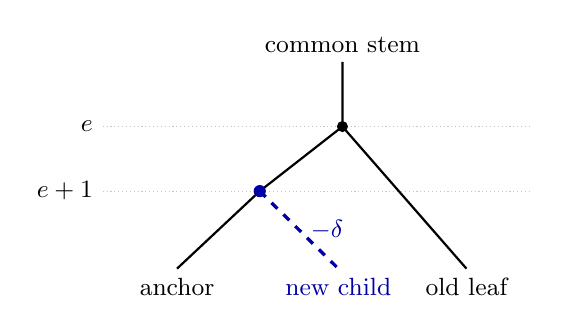
\begin{tikzpicture}[x=1.05cm,y=0.82cm,>=stealth,font=\small]
 \draw[gray!45,densely dotted] (-2.9,-1) -- (2.3,-1);
 \draw[gray!45,densely dotted] (-2.9,-2) -- (2.3,-2);
 \node[left] at (-2.9,-1) {$e$};
 \node[left] at (-2.9,-2) {$e+1$};
 \draw[thick] (0,0) -- (0,-1) -- (-1,-2) -- (-2,-3.2);
 \draw[thick] (0,-1) -- (1.5,-3.2);
 \draw[blue!65!black,very thick,dashed] (-1,-2) -- (-0.05,-3.2);
 \fill (0,-1) circle (2pt);
 \fill[blue!65!black] (-1,-2) circle (2.2pt);
 \node[above] at (0,0) {common stem};
 \node[below] at (-2,-3.2) {anchor};
 \node[below,blue!65!black] at (-0.05,-3.2) {new child};
 \node[below] at (1.5,-3.2) {old leaf};
 \node[right,blue!65!black] at (-0.5,-2.6) {$-\delta$};
\end{tikzpicture}
\caption{One local effect of delaying a target split. The old tree is solid;
the dashed child creates a split at the previously unary depth-$e+1$ vertex,
with coefficient $m_{e+1}-m_{e+2}=-\delta$.
The proof shifts every internal target depth and charges distinct vertices
separately, even when their depths coincide. Later target colors may reuse
eligible old leaves.}
\label{decor:shift-figure}
\end{figure}

Let $\kappa(T)$ be the reference coefficient \eqref{tree:K}, and put
\begin{equation}
 J=\kappa(S^+)^2.
 \label{decor:J-definition}
\end{equation}
At each
vertex the $j=1$ factor is $-\delta$; for $j\ge2$ its absolute value
is at least $\eta/2$ for all sufficiently large $L$.  If $b=b(S)$,
then
\begin{equation}
 |J|\ge c_{k,\eta}\delta^{2b}>0.
 \label{decor:J-lower-bound}
\end{equation}
For large $L$, regularity ensures that each shifted depth differs from
every branching depth of the old tree, including $d$. Thus these $2b$
target branching vertices must be created by fresh unary splits.
Lemma~\ref{tree:charging} gives
\begin{equation}
 \frac1{|J|}\sum_{\text{allowed extensions}}|c|
        \le C_{k,\eta}.
 \label{decor:relative-absolute-cost}
\end{equation}
The two copies have aligned depths but distinct branching vertices:
each vertex supplies its own factor $\delta$. This is the reason for
the shift. The full signed coefficient has an additional factor
$-\delta$ from separation at $d$; we divide by $J$ and leave that
factor in the identity. Equation~\eqref{decor:relative-absolute-cost}
then controls every projection error after division.

\paragraph{Projecting the two target sides.}
In every extension, the marginal target tree consists of two
ordinary copies of $S^+$, independent below their separation at $d$.
By \eqref{decor:projection-bound} its multioverlap differs in
$L^2$ from the contraction of its projected means at $e+1$ by at
most $2p_N(S^+,e+1)$.  Change the proper child depths back by one,
then change their evaluation depth from $e+1$ to $e$.  The product
difference inequality and Lemma~\ref{decor:depth-continuity} show
that this adds an error at most $h_N(S)$ in $L^2$, with
\begin{equation}
 \mathcal A_{L,\eta}h_N(S)^2\le C_k/L.
 \label{decor:projection-shift-error}
\end{equation}
One can take $h_N(S)$ to be the sum of the finitely many
$L^2(\|\cdot\|_N)$ distances in these comparisons, multiplied by
a size-dependent constant.  This definition depends only on the
single-copy marginal shapes, not on the particular extension.
Thus \eqref{decor:projection-shift-error} holds uniformly for the
comparisons in the extension sum, even though the union of the
old and target trees itself need not have regular depths.

Let $a,b$ denote the vectors $a_{S,e}$ on the old stems I and II.
The target stem in I shares the old prefix through $e$ because it
contains the anchor, so its final projected vector is $a$.

\paragraph{The signed extension sum.}
Set $f$ to be the overlap of all $2k$ old leaves, an allowed fixed
overlap monomial. All target-I additions stay in the anchor's branch
below $d$, so they leave the old-II stem and its child counts unchanged.
Classify the first added path of target side II by its prefix
through $e$.  It may diverge freshly at $\ell=d$, with coefficient
$-c_d$, or follow the old II stem and diverge at $d<\ell<e$, with
coefficient $-c_\ell=-\delta$.  In such a class let $b_\ell$ be
$a_{S,e}$ on the new stem; it shares the old II prefix through
$\ell$.  At $\ell=d$ the stems carrying $a,b,b_d$ are conditionally
independent below $d$.  Every remaining possibility follows the
old II prefix through $e$ and has final projected vector $b$.
All later target paths in side II follow its first path through
$e$, since their earliest split is $e+1$.

For a fixed extension history, retain every old path and the first
target-II prefix through $e$, and delete all other new branches.
The target-I projection $a$ already depends only on the retained old
anchor prefix. Each deleted subtree integrates to one under its
probability kernels; a reused old leaf introduces no new variable.
The retained tree depends only on the class: it is the old tree with a
fresh stem attached at $\ell<e$, or just the old tree in the remaining
class. The history is a combinatorial choice, not a condition on sampled
values. Thus the joint marginal of the old paths and projected prefixes
is fixed within each class. In particular, the expectation of $f$ times
the projected overlap is constant within a class and can be multiplied
by its total signed coefficient.

By Lemma~\ref{tree:reference-total}, summing later side-II colors
backwards gives $\kappa(S^+)$ for each first-path choice.  Summing the
side-I choices gives the other factor $\kappa(S^+)$. The fresh class
at $\ell$ therefore has total coefficient $-c_\ell J$.
The total coefficient is $-\delta J$, both from the old tree and
from the anchor alone. Since
\[
 \sum_{\ell=d}^{e-1}c_\ell=(e+1)\delta=m_e+\delta,
\]
the remaining prefix-through-$e$ class has coefficient $m_eJ$.
Thus the projected terms have the following coefficients:
\[
 \begin{array}{c|c|c}
 \text{side-II prefix} & \text{projected overlap}
      & \text{total coefficient}\\ \hline
 \text{fresh divergence at }d\le\ell<e & a\cdot b_\ell & -c_\ell J\\
 \text{old prefix through }e & a\cdot b & m_eJ
 \end{array}
\]

Multiply the projected overlap in each row by $f$ and divide the
prescribed-tree identity by $J$. Rearranging gives
\begin{equation}
 \sum_{\ell=d}^{e-1}c_\ell
   \mathbb E\bigl[f(a\cdot b-a\cdot b_\ell)\bigr]
 =\delta\bigl(\mathbb E[f(a\cdot b)]
          -\mathbb Ef\,\mathbb ER_{\mathrm{target}}\bigr)
       +\rho_N(S,d),
 \label{decor:induction-identity}
\end{equation}
where $R_{\mathrm{target}}$ on the right is the target overlap in
the anchor-alone extension.  Its absolute value is at most one.
The error satisfies
\begin{equation}
 |\rho_N(S,d)|\le C_{k,\eta}
       \bigl(p_N(S^+,e+1)+h_N(S)\bigr)
       +C_{L,k,\eta}\varepsilon_{N,L,k}.
 \label{decor:induction-error}
\end{equation}
Indeed, multiplying a projection error by $f$, even when correlated
with it, costs at most its $L^2$ norm since $|f|\le1$. Sum these errors
with absolute coefficients and apply
\eqref{decor:relative-absolute-cost}. The final term includes division
of the original identity error by $J$ and tends to zero at fixed $L$.

\paragraph{Closing the induction.}
Equation~\eqref{decor:projection-bound} gives
$\|f-a\cdot b\|_{L^2}\le2p_N(S,e)$.
Moreover
$\sum_{\ell=d}^{e-1}c_\ell=(e+1)\delta\le1$.
Replacing $f$ by $a\cdot b$ on the left of
\eqref{decor:induction-identity} therefore costs at most
$4p_N(S,e)$.  Each $a\cdot b_\ell$ has the same marginal law as
$a\cdot b$, so that left side becomes
\[
 \frac12\sum_{\ell=d}^{e-1}c_\ell
        \mathbb E(a\cdot b-a\cdot b_\ell)^2.
\]
Its summands are nonnegative and $c_d\ge\eta$.  The right side
of \eqref{decor:induction-identity} is bounded in absolute value
by $2\delta+|\rho_N(S,d)|$.  Hence
\begin{equation}
 \mathbb E(a\cdot b-a\cdot b_d)^2
 \le C_\eta\bigl(\delta+p_N(S,e)+|\rho_N(S,d)|\bigr).
 \label{decor:projected-three-copy}
\end{equation}
Sample three copies of $A_S$ conditionally independently below
$d$.  Projecting each of the two contractions involving the
first copy changes it in $L^2$ by at most $2p_N(S,e)$.
Using \eqref{decor:three-copy-bound},
\eqref{decor:projected-three-copy}, and $p_N(S,e)\le k$, we obtain
\begin{equation}
 v_N(S,d)\le C_{k,\eta}\bigl(
       \delta+p_N(S,e)+p_N(S^+,e+1)+h_N(S)\bigr)
       +C_{L,k,\eta}\varepsilon_{N,L,k}.
 \label{decor:covariance-induction-estimate}
\end{equation}
Each child in either $p_N$ has fewer than $k$ leaves. To make the
averaging step explicit, the aligned construction has
$D=b(S)+1$ distinct depth coordinates, including $d$ and $e$.
A term belonging to $T_j$ uses only $D_j=b(T_j)+1$ coordinates.
For the shifted term these are
$\pi_j(\mathbf q)=(e+1,(q_v+1)_{v\in\operatorname{Br}(T_j)})$.
Every retained assignment has at most $L^{D-D_j}$ preimages, and its
coordinates are $\eta/2$-regular for large $L$. If $w_j$ is the child
covariance as a function of these coordinates, then, for $0<\gamma\le1$,
\begin{align}
 L^{-D}\sum_{\mathbf q\;\eta\text{-regular}}
       w_j(\pi_j(\mathbf q))^\gamma
 &\le L^{-D_j}\sum_{\mathbf y\;\eta/2\text{-regular}}w_j(\mathbf y)^\gamma
 \notag\\
 &\le\left(L^{-D_j}\sum_{\mathbf y\;\eta/2\text{-regular}}
       w_j(\mathbf y)\right)^\gamma.
 \label{decor:fiber-bound}
\end{align}
The unshifted term has the same bound without translating the coordinates.
Thus the two aligned copies use single-copy estimates; there is no
restriction of an independently averaged pair of copies to a diagonal.
Taking $\gamma=1/4$ and then $\limsup_N$, and using
\eqref{decor:projection-shift-error} and
\eqref{decor:identity-error}, gives, for sufficiently large $L$,
\begin{equation}
 V_{k,L}(\eta)\le C_{k,\eta}\left(
       L^{-1/2}+V_{k-1,L}(\eta/2)^{1/4}\right).
 \label{decor:induction-recursion}
\end{equation}
The maximum over smaller topologies in \eqref{decor:V-definition}
can be absorbed in the right side because these covariances are
bounded by one.  The base case and induction now imply
$V_{k,L}(\eta)\to0$ for every fixed $k,\eta$, proving the proposition.
\end{proof}

\subsection{Concentration of every multioverlap}

The covariance estimate controls fluctuations below a sampled prefix.
We now use a marker anchor to concentrate the prefix projection, and
combine this with the averaged continuity estimate.

\begin{proof}[Proof of \cref{decor:overlap-concentration}]
For a singleton, use the spin-anchor identity with no added colors
and $f=R_S$.  It gives
$\mathbb ER_S^2=(\mathbb ER_S)^2+o_N(1)$.

Suppose $S$ first splits at $e$ and has proper child shapes
$T_1,\ldots,T_s$. We will condition one step before $e$. Use $S$ as
the old tree, designate one of its
leaves as a marker anchor, and add a full copy of $S$ all of whose
leaves split from the anchor at $e-1$.  Its first path must be
fresh at $e-1$, because the old tree has not yet branched there.
All other target paths lie in the resulting fresh subtree.
The extension coefficient on both sides of the prescribed-tree
identity is the same nonzero number
\begin{equation}
 C(S,e)=-\delta \kappa(S).
 \label{decor:marker-coefficient}
\end{equation}
The target and old copies are conditionally independent and
identically distributed below $\mathscr F_{e-1}$. With
$f=R_S$ and $M=\mathbb E[R_S\mid\mathscr F_{e-1}]$, their product has
conditional expectation $M^2$. On the anchor-alone side, deleting the
marker's continuation below $e-1$ integrates a probability kernel to one
and leaves the ordinary target law $S$, with mean $\mathbb E R_S$.
The identity therefore gives
\begin{equation}
 C(S,e)\bigl(\mathbb EM^2-(\mathbb E R_S)^2\bigr)
 =C(S,e)\operatorname{Var}(M)=o_N(1),
 \label{decor:marker-variance-identity}
\end{equation}
and hence
\begin{equation}
 \qquad \operatorname{Var}(M)\longrightarrow0
 \quad\text{at each fixed }L,S,e.
 \label{decor:prefix-projection-concentration}
\end{equation}
Division by $C(S,e)$ is made only at fixed $L$; no uniform lower
bound as $L\to\infty$ is needed.

It remains to control the conditional variance below this prefix.
The child covariances are evaluated at $e$, which is separated from
all their branching depths; the move to $e-1$ will use martingale
continuity instead. Set
\[
 G=\mathbf1\cdot\prod_j \mu_{e,T_j},
 \qquad G_-=\mathbf1\cdot\prod_j \mu_{e-1,T_j}.
\]
The latter is $\mathscr F_{e-1}$-measurable.  By
\eqref{decor:projection-bound},
$\mathbb E(R_S-G)^2\le p_N(S,e)^2$.
Keeping all proper child depths fixed, the product difference
inequality and \eqref{decor:martingale-energy} imply
\begin{equation}
 \mathcal A_{L,\eta}\mathbb E(G-G_-)^2\le C_k/L.
 \label{decor:adjacent-prefix-error}
\end{equation}
Here $e$ is itself a ranged coordinate, so the one-step increments
are summed before division by $L$.  Since conditional expectation
is the optimal $L^2$ projection,
\[
 \mathbb E(R_S-M)^2
   \le\mathbb E(R_S-G_-)^2
   \le2p_N(S,e)^2+2\mathbb E(G-G_-)^2.
\]
Variance decomposition and
\eqref{decor:prefix-projection-concentration} now show
\begin{equation}
 \limsup_{N\to\infty}
      \mathcal A_{L,\eta}\operatorname{Var}(R_S)
 \le C_k\left(L^{-1}+V_{k-1,L}(\eta/2)^{1/2}\right)
 \quad\text{for all sufficiently large }L.
 \label{decor:variance-estimate}
\end{equation}
In this estimate we used
$p_N(S,e)^2\le s\sum_jv_N(T_j,e)^{1/2}$ and
\eqref{decor:fiber-bound} with $\gamma=1/2$: here the full average has
$D=b(S)$ coordinates because $d$ is absent, while still
$D_j=b(T_j)+1$. Proposition~\ref{decor:conditional-concentration}
finishes the proof.
\end{proof}

\begin{remark}
\label{decor:order-of-limits}
All uncancelled small denominators in this section occur only in prescribed-tree
identity errors.  At fixed $L$ there are finitely many relevant trees,
so those errors disappear before any depth average or $L$ limit is
taken.  Errors that survive the $N$ limit are controlled by the
uniform relative absolute-cost bound
\eqref{decor:relative-absolute-cost}, the lower-order covariance
averages, and the martingale estimate $C/L$.  No rate of convergence
in $N$ uniform in $L$ is used.
\end{remark}
